\section{Power Generation}
\begin{itemize}
 \item individual atoms have discrete energy levels
 \item probability of occupation at energy E
 \[f(E) = \frac{1}{1+e^{\frac{E-E_F}{kT}}}\]
 \item current is conducted via electrons in the conduction band (electrons)
 \item since there are vacant positions in the valence band, the electrons there can contribute to the current as well (holes)
 \item electrons and holes are treated as quasi free particles
 \item doping of semiconductors: replace a group of atoms by a group of atoms with lower or higher ordinal number (acceptors/donors)
 \item n-doped: higher ordinal number, p-doped: lower ordinal number
 \item so far: semiconductor in equilibrium, now: under illumination
 \item energy of light is added to the electron's energy which can lift the electron from the valence band to the conduction band
 \item recombination:
 \begin{itemize}
  \item light creates electron hole pairs
  \item if light is switched off: recombination
  \item but also present: radiative recombination (cannot be prevented)
 \end{itemize}
 \item pn junction: bring p- and n- doped semiconductor in contact
 \item upon forming the junction, there is a large concentration gradient and an associated diffusion current from holes leaving the p region and e- leaving the n region
 \item at the same time, a space charge is created by the ionized dopant atoms, in the resulting electrical field an opposing drift current develops
 \item in equilibrium, both currents are equal (for e- as well as holes) and no net current flows
 \item pn-junction under illumination = solar cell
 \item Summary solar cell principles
 \begin{itemize}
  \item a semiconductor has a gap in the energy band diagram
  \item at T$>$0 free charge carriers (electrons, holes) exist
  \item by doping, one type is increased dramatically which leads to the distinction majority/minority carrier
  \item under illumination, minority carriers are created
  \item due to the fact that there is a gap in the allowed energy levels, they don’t relax immediately but have a finite lifetime $\uptau$
  \item if they can be extracted before they recombine, they provide an external current $\Rightarrow$ solar cell
  \item a pn junction does exactly that. The built-in field creates an asymmetry in the band structure. Majority carrier cannot cross it, but minority carriers can.
  \item if a charge carrier crosses the pn junction, it is transformed from a minority carrier (e.g. e- in the p doped material into a majority carrier in the n doped side) with 
  essentially infinite lifetime
 \end{itemize}
\end{itemize}

\subsection{solar cell basics}
For real solar cells, the following idealizations are not valid any more:
\begin{itemize}
 \item infinite cell dimensions: real solar cells have surfaces, which are ideal recombination sites
 \item homogeneous carrier generation G: the absorption is wavelength and depth dependent (longer wavelength has larger penetration depth)
 \item recombination in the depleted region cannot always be neglected
\end{itemize}
Typically, the I-V curves are plotted in the first quadrant. Key parameters describing the IV curve:
\begin{itemize}
 \item ppen circuit voltage $V_{oc}$
 \item short circuit current $I_{sc}$
 \item maximum power ($P_{max}$ – $V_{mp}$/$I_{Mp}$)
\end{itemize} 
\begin{figure}[!ht]
 \centering
 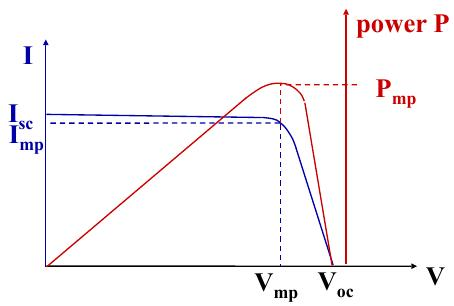
\includegraphics[scale=0.5]{solarcell}
\end{figure}

\subsection{solar cells for space}
Main requirements:
\begin{itemize}
 \item high efficiency
 \item low mass
 \item radiation resistant
\end{itemize}
Evolution: Si cells $\Rightarrow$ cells based on direct semiconductors $\Rightarrow$ multijunction cells.\\
\vspace*{3pt}

\noindent \textbf{multijunction cells}
\begin{itemize}
 \item efficiency of Si cells: 18\%
 \item additional junction reduces thermalization losses and increases efficiency $\Rightarrow$ multijunction cells
\end{itemize}
\begin{figure}[!ht]
 \centering
 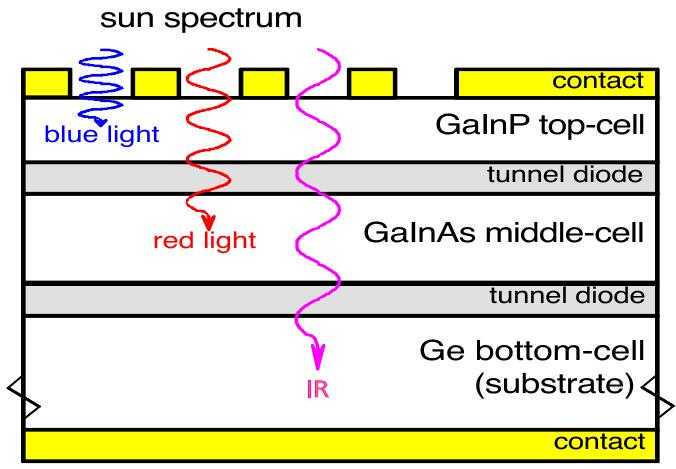
\includegraphics[scale=0.5]{triplejunction}
\end{figure}

\subsection{solar array technology}
\textbf{radiation environment in space}:
\begin{itemize}
 \item protons and electrons trapped in the earth magnetic field 
 \item solar protons 
\end{itemize}
\textbf{damage caused by particle radiation}:
\begin{itemize}
 \item ionization damage
 \item displacement damage 
\end{itemize}
\textbf{matching of solar cells}:
\[\text{current}I(S) = \sum I_{\nu}(U)\]
\[\text{voltage}V(S) = \sum V_{\mu}(I)\]
\[I(S) = n\cdot I_{cell}\]
\[V(S) = m\cdot V_{cell}\]
\textbf{power prediction}
\begin{enumerate}
 \item mission profile
 \begin{itemize}
  \item launch date
  \item launcher
  \item transfer orbits
  \item final orbit
  \item lifetime
  \item power requirements and power profile
  \item solar array orientation
 \end{itemize}
 \item satellite configuration
 \begin{itemize}
  \item power control and power conditioning (fixed voltage or maximum power tracking)
  \item solar generator type (body mounted, deployable fixed or sun oriented)
 \end{itemize}
 \item main parameters derived from orbit
 \begin{itemize}
  \item intensity and incidence angle of sun insolation over mission time
  \item effective Earth/planet radiation and albedo
  \item type, spectrum and intensity of charged particle irradiation
  \item loss factors BOM and EOM
  \item optimum solar cell and coverglass type
 \end{itemize}
\end{enumerate}
\textbf{power limiting factors} 
\vspace*{3pt}

\noindent basic and design related:
 \begin{itemize}
  \item temperature
  \item calibration inaccuracy
  \item mismatch
  \item coverglass gain/loss
  \item cable losses
  \item random failures
 \end{itemize}

\noindent mission related:
 \begin{itemize}
  \item sun intensity
  \item irradiation angle
  \item charged particles 
  \item micrometeorites/debris
 \end{itemize}
\textbf{mechanical solar array design} 
\vspace*{3pt}

\noindent so far: situation in orbit, now: mechanical criteria during satellite launch
 \begin{itemize}
  \item it has to be folded to the satellite sidewall in order to fit inside the launch vehicle
  \item it has to supply power during transfer orbit ($\rightarrow$ partial deployment)
  \item it has to be fully deployed once in geosynchronous orbit
  \item the mechanical design has to survive the acoustic loads (created by the main engines of the launch vehicle, reflected from the launch pad) and vibrational loads
 \end{itemize}
